\documentclass[11pt]{article}
\usepackage[scaled=0.92]{helvet}
\usepackage{geometry}
\geometry{letterpaper,tmargin=1in,bmargin=1in,lmargin=1in,rmargin=1in}
\usepackage[parfill]{parskip} % Activate to begin paragraphs with an empty line rather than an indent %\usepackage{graphicx}
\usepackage{amsmath,amssymb, mathrsfs, dsfont}
\usepackage{tabularx}
\usepackage[font=footnotesize,labelfont=bf]{caption}
\usepackage{graphicx}
\usepackage{xcolor}
%\usepackage[linkbordercolor ={1 1 1} ]{hyperref}
%\usepackage[sf]{titlesec}
\usepackage{natbib}
\usepackage{../../Tianpei_Report}
%\usepackage{appendix}
%\usepackage{algorithm}
%\usepackage{algorithmic}

%\renewcommand{\algorithmicrequire}{\textbf{Input:}}
%\renewcommand{\algorithmicensure}{\textbf{Output:}}



\begin{document}
\title{Lecture 5: Dependency Parsing}
\author{ Tianpei Xie}
\date{ Jul. 4th., 2022 }
\maketitle
\tableofcontents
\newpage
\allowdisplaybreaks
\section{Concepts}
There are two major categories of grammar study:
\begin{itemize}
\item \textbf{Phrase-Structure Grammars}: discussed in previous chapters. It focuses on \emph{constituency structures and relations}, groups of words can behave as single units.  Part of developing a grammar involves building an inventory of the constituents in the language. The constituents can be placed in one place together but not individual word within it.

\item \textbf{Dependency Grammars (DG)}: focuses on the \emph{dependency} relation (as opposed to the \emph{constituency relation} of \emph{phrase structure}). In dependency formalisms, phrasal constituents and phrase-structure rules \emph{do not play a direct role}. Instead, the syntactic structure of a sentence is described \emph{solely} in terms of \textbf{\emph{directed binary} grammatical \emph{relations}} between the words
\end{itemize}

\begin{figure}
\begin{minipage}[t]{1\linewidth}
  \centering
  \centerline{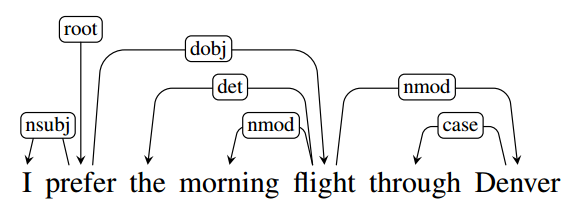
\includegraphics[scale = 0.5]{dependent_parse_tree.png}}
\end{minipage}
\caption{\footnotesize{\textbf{An example dependent parse tree}.}}
\label{fig: dep_parse_tree}
\end{figure}

An example of dependency parse tree is illustrated in Figure \ref{fig: dep_parse_tree}. Relations among the words are illustrated above the sentence with \emph{directed, labeled arcs} from heads to dependents. We call this a \textbf{typed dependency structure} because the labels are drawn from a \emph{fixed inventory} of grammatical relations. A \textbf{root} node explicitly marks the root of the tree, the \textbf{head} of the entire structure.

Note the absence of nodes corresponding to phrasal constituents or lexical categories in the dependency parse; the internal structure of the dependency parse consists solely of
directed relations between lexical items in the sentence. These \textbf{head-dependent relationships} directly encode important information that is often buried in the more
complex phrase-structure parses. 

A major \textbf{advantage} of dependency grammars is their ability to deal with languages that are \emph{morphologically} rich and have a relatively \textbf{free word order}. The same type of dependent relation but with different word ordering may require different rules in phase structure grammar. Thus, a dependency grammar approach abstracts away from \emph{word order information}, representing only the information that is necessary for the parse.

An additional practical motivation for a dependency-based approach is that the \textbf{head-dependent relations} provide an approximation to the \emph{\textbf{semantic relationship}} between \textbf{predicates} and their \textbf{arguments} that makes them directly useful for many applications such as \emph{coreference resolution}, \emph{question answering} and \emph{\textbf{information extraction}}. Constituent-based approaches to parsing provide similar information, but it
often has to be \emph{distilled} from the trees via techniques such as the \textbf{head-finding rules}.


Figure \ref{fig: dep_constit_tree} shows the difference between a dependency parse tree and a constituency parse tree for the same sentence. In constituency parse tree, only leaves represent the words, and the internal non-terminal nodes are phase structures. In dependency parse tree, the edges (dependency relation) are directed links from one word to another word. In graph perspective, the dependency tree is homogenous graph with nodes all representing words, while the constituency parse tree is heterogenous graph with terminal nodes representing words and non-terminal nodes representing abstract phrases. 

\begin{figure}
\begin{minipage}[t]{1\linewidth}
  \centering
  \centerline{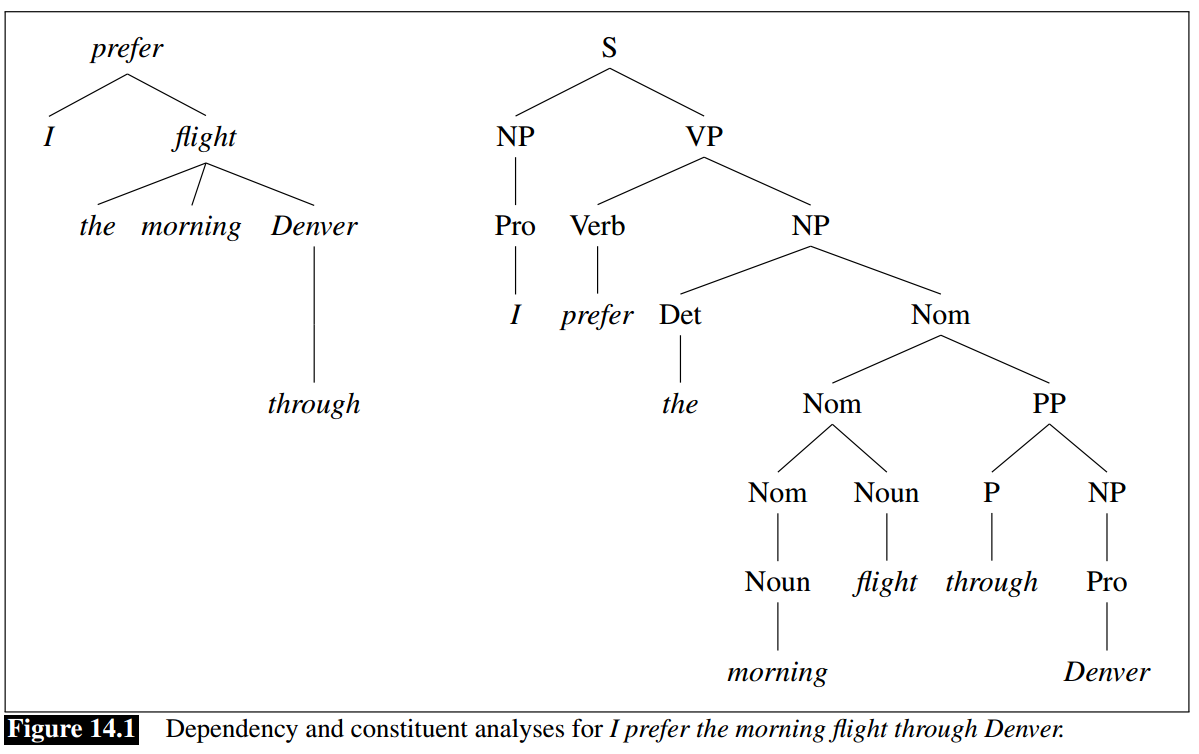
\includegraphics[scale = 0.3]{dep_constit_tree.png}}
\end{minipage}
\caption{\footnotesize{\textbf{A comparison between the dependency parse tree and constituency parse tree}.}}
\label{fig: dep_constit_tree}
\end{figure}

\section{Dependent relations}
The traditional linguistic notion of \textbf{grammatical relation} provides the basis for the binary relations that comprise these dependency structures. The arguments to these relations consist of a \textbf{head} and a \textbf{dependent}.
\begin{itemize}
\item  the \textbf{head} word of a constituent was the central organizing word of a larger constituent (e.g, the primary noun in a noun phrase, or verb in a verb phrase). 

\item The remaining words in the constituent are either direct, or indirect, \textbf{dependents} of their head. 
\end{itemize}
In dependency-based approaches, the head-dependent relationship is made explicit by directly \textbf{linking} \textbf{heads} to the words that are \textbf{immediately dependent} on them, bypassing the need for constituent structures. It also classify different kinds of grammatical relations, or \textbf{grammatical function} that the
dependent plays with respect to its head. These include familiar notions such as \emph{subject}, \emph{direct object} and \emph{indirect object}. Note that in English, hese notions strongly correlate with, but by no means determine, both position in a sentence and constituent type and are therefore somewhat \emph{redundant} with the kind of information found in phrase-structure trees.

The \textbf{Universal Dependencies (UD)} project \citep{nivre2016universal} provides an inventory of dependency relations that are linguistically motivated, computationally useful, and cross-linguistically applicable. Figure \ref{fig: dep_relation} provides a subset of the UD relations. The core set of frequently used relations can be
broken into two sets: 
\begin{itemize}
\item \textbf{clausal relations} that \emph{describe syntactic roles} with respect to a \emph{predicate (often a verb)}; and
\item \textbf{modifier relations} that categorize the ways that words can \emph{modify} their heads.
\end{itemize}
  
\begin{figure}
\begin{minipage}[t]{1\linewidth}
  \centering
  \centerline{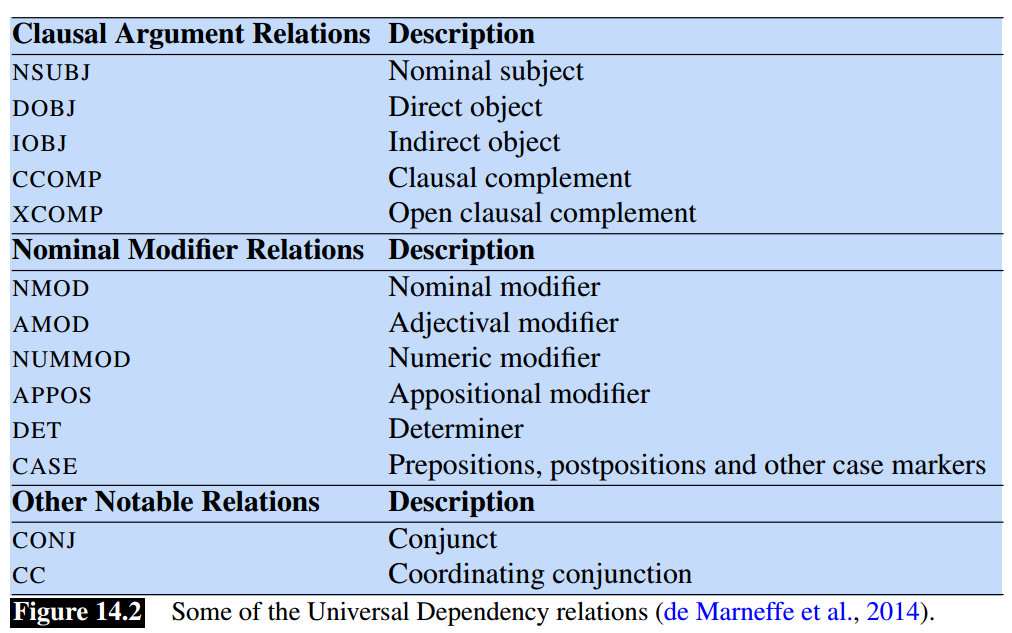
\includegraphics[scale = 0.3]{dep_relations.png}}
\end{minipage}
\caption{\footnotesize{\textbf{Some depedent relation tags}.}}
\label{fig: dep_relation}
\end{figure}

\subsection{Dependency Formalisms}
A dependency structure can be represented as a directed graph $G = (V,A)$, consisting of a set of vertices $V$, and a set of ordered pairs of vertices $A$, which we’ll call \emph{arcs}. $V$ is the set of words in a sentence and $A$ captures the headdependent and grammatical function relationships between the elements in $V$.

A \textbf{dependency tree} is a \emph{directed} graph that satisfies the following constraints:
\begin{enumerate}
\item There is a \emph{single} designated \textbf{root} node that has no incoming arcs. (\textbf{single head})
\item With the exception of the root node, each vertex has \textbf{exactly one incoming arc}. (\textbf{connected})
\item There is a \textbf{unique path} from the root node to each vertex in $V$.
\end{enumerate}

The notion of \textbf{projectivity} imposes an additional constraint that is derived from the order of the words in the input.  An arc from a head to a dependent is said to be
\textbf{projective}  if there is a path from the head to every word that lies between the head and the dependent in the sentence.  \textbf{A dependency tree} is then said to be \textbf{projective} if \textbf{all} the arcs that make it up are projective.

As we can see from the diagram Figure \ref{fig: dep_parse_tree}, projectivity (and non-projectivity) can be detected in the way we’ve
been drawing our trees. A dependency tree is \emph{projective} if it can be drawn with \textbf{no crossing edges}. The dependency tree generated from constituent tree in the TreeBank using \emph{head-finding rule} is projective. Also some of commonly used algorithms can only generate projective dependency parse tree. 
The translation process from constituent to dependency structures has two \emph{subtasks}: identifying all the \emph{\textbf{head-dependent relations}} in the structure and identifying the \textbf{correct dependency relations} for these relations. The head-finding rules are used for the first task. Here’s a simple and effective algorithm
\begin{enumerate}
\item Mark the head child of each node in a phrase structure, using the appropriate head rules.
\item In the dependency structure, make the \emph{head} of each \emph{non-head child} depend on the \emph{head of the head-child}.
\end{enumerate}

\section{Transition-Based Dependency Parsing}
Our first approach to dependency parsing is called \textbf{transition-based parsing}. This architecture draws on \textbf{\emph{shift-reduce parsing}}, a paradigm originally developed for analyzing programming languages. In transition-based parsing we’ll have a \textbf{stack} on which we build the parse, a \textbf{buffer} of tokens to be
parsed, and a \textbf{parser} which takes actions on the parse via a predictor called an \textbf{oracle}. Figure \ref{fig: shift_reduce_parse} illustrates the architecture of the shif-reduce parser. 


\begin{figure}
\begin{minipage}[t]{1\linewidth}
  \centering
  \centerline{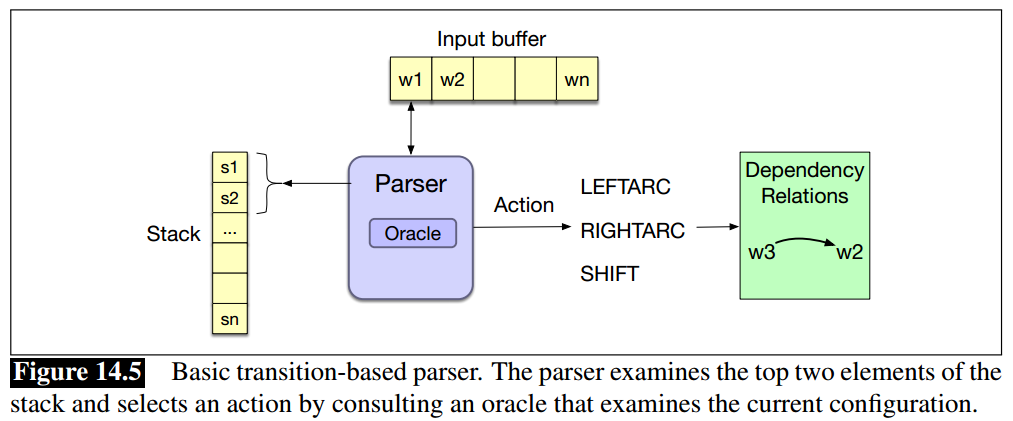
\includegraphics[scale = 0.4]{shift_reduce_parse.png}}
\end{minipage}
\caption{\footnotesize{\textbf{The architecture of shift-reduce parser}.}}
\label{fig: shift_reduce_parse}
\end{figure}

The parser walks through the sentence left-to-right, successively \emph{shifting} items from the buffer onto the stack. At each time point we examine the \textbf{top two elements} on the stack, and the oracle makes a decision about what \textbf{transition} to apply to build the parse. The possible transitions correspond to the \emph{intuitive actions} one might take in creating a dependency tree by examining the words in \emph{a single pass} over the input from left to right:
\begin{itemize}
\item Assign the current word as the \emph{head} of some \emph{previously seen} word;
\item Assign some previously seen word as the \emph{head} of the \emph{current} word;
\item \emph{Postpone} dealing with the current word, \emph{storing} it for later processing
\end{itemize} We’ll formalize this intuition with the following three transition operators that will operate on the top two elements of the stack:
\begin{itemize}
\item \textbf{LEFTARC}: \textbf{Assert} a head-dependent relation between the word at the \emph{\textbf{top}} of the \textbf{stack} and the \emph{second} word; \emph{\textbf{remove}} the \textbf{second} word from the stack.
\item  \textbf{RIGHTARC}: \textbf{Assert} a head-dependent relation between the \textbf{second} word on the \textbf{stack} and the word at the \emph{top}; \emph{\textbf{remove}} the \textbf{top} word from the stack;
\item  \textbf{SHIFT}: \textbf{Remove} the word from the front of the input buffer and \textbf{push} it onto the stack.
\end{itemize}
We’ll sometimes call operations like LEFTARC and RIGHTARC \textbf{reduce operations}, based on a metaphor from shift-reduce parsing, in which reducing means combining elements on the stack. There are some \emph{preconditions} for using operators. The LEFTARC operator cannot be applied when \textbf{ROOT} is the \emph{second} element of the stack (since by definition the ROOT node cannot have any incoming arcs). And both the LEFTARC and RIGHTARC operators require \textbf{two elements to be on the stack} to be applied.

This particular set of operators implements what is known as the \textbf{arc standard approach} to transition-based parsing. In arc standard
parsing the transition operators only assert relations between elements at the \emph{top of the stack}, and once an element has been assigned its \emph{head} it is \emph{removed} from the stack and is not available for further processing. 

\begin{figure}
\begin{minipage}[t]{1\linewidth}
  \centering
  \centerline{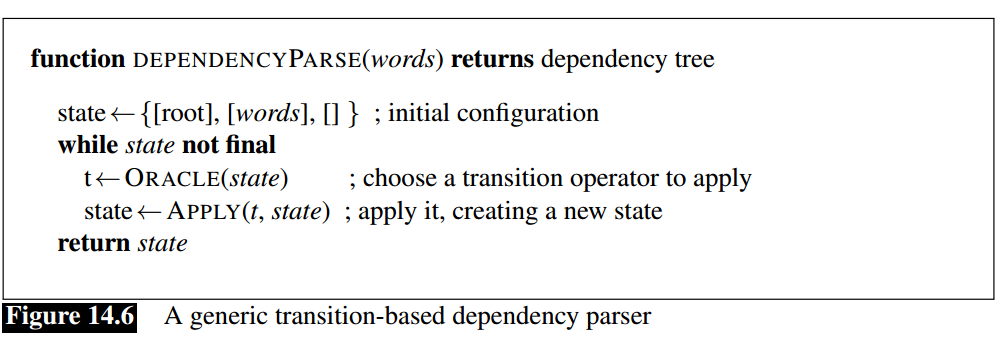
\includegraphics[scale = 0.4]{transit_based_parser.png}}
\end{minipage}
\caption{\footnotesize{\textbf{The algorithm for transit-based parser}.}}
\label{fig: transit_based_parser}
\end{figure}

The specification of a transition-based parser is quite simple, based on representing the current \textbf{state} of the parse as a \textbf{configuration}: the \emph{\textbf{stack}}, an \emph{\textbf{input buffer}} of words or tokens, and a set of \textbf{\emph{relations}} representing a dependency tree. \emph{Parsing}
means making a \textbf{sequence of transitions through the space of possible configurations}. We start with an \textbf{initial configuration} in which the stack contains the \emph{ROOT} node, the buffer has the tokens in the sentence, and an \emph{empty set of relations} represents the parse. In the \textbf{final goal state}, the \emph{stack} and the \emph{word list} should be \emph{\textbf{empty}}, and the set of relations will represent the \textbf{final parse}. Figure \ref{fig: transit_based_parser} provides the algorithm description.  The process \textbf{ends} when all the words in the sentence have been consumed and \textbf{the ROOT node is the only element remaining on the stack}.

The efficiency of transition-based parsers should be apparent from the algorithm. The complexity is \textbf{linear} in the length of the sentence since it is based on a single
left to right pass through the words in the sentence. (Each word must first be shifted onto the stack and then later reduced.) Unlike the dynamic programming algorithm for constituency parsing, the transition-based dependency parser is \textbf{greedy algorithm}.  The oracle provides a \emph{single choice} at each step and the parser proceeds with that choice, no other options are explored, no backtracking is employed, and a single parse is returned in the end.

There are several important things to note when examining sequences during the parsing. First, the sequence given is \textbf{not the only one} that might lead to a reasonable parse.  In general, there may be \textbf{more than one path} that leads to the same result, and due to \emph{ambiguity}, there may be other transition sequences that lead
to different equally valid parses.  Second, we are assuming that the \textbf{oracle} always provides the correct operator at each point in the parse—an assumption that is unlikely to be true in practice. As a result, given the greedy nature of this algorithm, incorrect choices will lead to incorrect parses since the parser has no opportunity to go back and pursue alternative choices. 

\subsection{Creating an Oracle}\label{sec: train_model}
The oracle for greedily selecting the appropriate transition is trained by supervised machine learning. The oracle from the algorithm in Figure \ref{fig: transit_based_parser} takes as input a \emph{configuration} and returns a \emph{transition operator}. Therefore, to train a classifier, we will need configurations paired
with transition operators (i.e., \emph{LEFTARC}, \emph{RIGHTARC}, or \emph{SHIFT}). Unfortunately, treebanks pair entire sentences with their corresponding trees, not configurations with transitions.

To generate the required training data, we supply our oracle with the \textbf{training sentences} to be parsed \emph{along with} their \textbf{corresponding reference parses} from the treebank. To produce training instances, we then \textbf{simulate} the operation of the parser by running the algorithm and relying on a new \textbf{training oracle} to give us correct transition operators for each successive configuration.

To be more precise, define $V$ as a set of vertices in the dependency tree (words), $R_{p}$ as a set of dependency relations. The \textbf{reference parse} consists of $(V, R_{p})$. The current \textbf{configuration} is defined as $(S, R_{c})$ where $S$ represents the stack and $R_{c}$ represents a set of current dependency relations.  Given a \textbf{reference parse} $(V, R_{p})$ and a \textbf{configuration} $(S, R_{c})$, the training oracle proceeds as follows:
\begin{itemize}
\item Choose \emph{\textbf{LEFTARC}} if it produces a \emph{correct head-dependent relation} given the reference parse and the current configuration, 
\begin{align*}
S_1\;\;r \;\; S_2 & \in R_{p}
\end{align*} where $S_1, S_2 \in S$.
\item  Otherwise, choose \textit{\textbf{RIGHTARC}} if (1) it produces a correct head-dependent relation given the reference parse \textbf{and} (2) all of the \emph{dependents} of the word at the \textbf{top} of the stack \emph{have already been assigned},
\begin{align*}
S_2\;\;r \;\; S_1 & \in R_{p} \;\; \\
\text{and }\forall\,r^{'},w,\quad \text{if }S_1\;\;r^{'} \;\; w & \in R_{p},\;\;\text{ then }S_1\;\;r^{'} \;\; w \in R_{c}
\end{align*} where $S_1, S_2 \in S$.
\item Otherwise, choose \emph{\textbf{SHIFT}}.
\end{itemize} The restriction on RIGHTARC is to make sure that a word is not popped from the stack, and thus lost to further processing, \emph{before} all its
dependents have been assigned to it.

\begin{figure}
\begin{minipage}[t]{1\linewidth}
  \centering
  \centerline{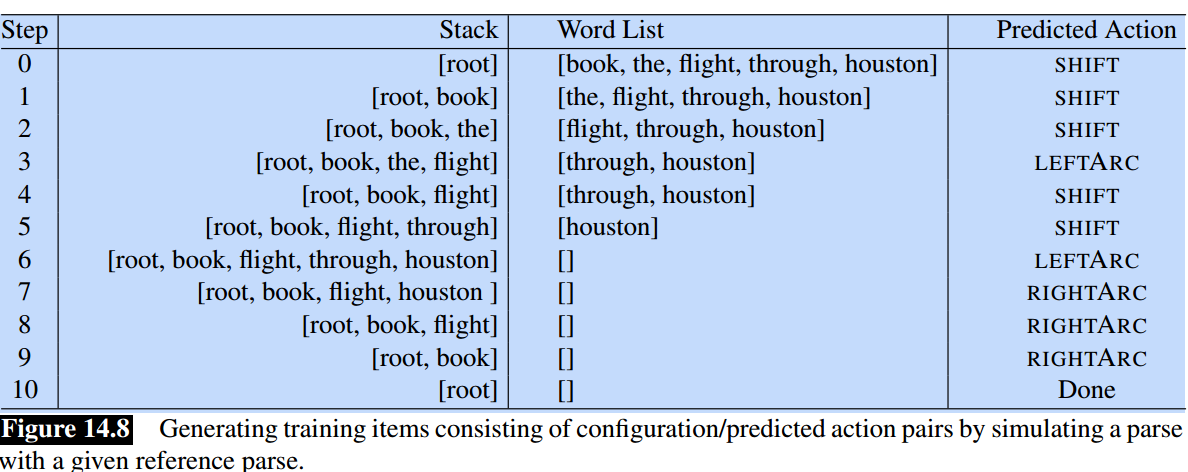
\includegraphics[scale = 0.4]{dep_parse_training_sample.png}}
\end{minipage}
\caption{\footnotesize{\textbf{The training samples are generated from reference parse}.}}
\label{fig: dep_parse_training_sample}
\end{figure}


\subsection{Feature-based classifier}\label{sec: feature_classifier}
Featured-based classifiers generally use the same features we’ve seen with part-of-speech tagging and partial parsing: \emph{Word forms}, \emph{lemmas}, \emph{parts of speech}, the \emph{head}, and the \emph{dependency relation to the head}. The features are extracted from the \emph{training configurations}, which consist
of the \emph{stack}, the \emph{buffer} and the \emph{current set of relations}. We can use the \textbf{feature template} that we introduced for sentiment analysis and
part-of-speech tagging. Feature templates allow us to automatically \emph{generate} large numbers of specific features from a training set. 
\begin{align*}
<s_1.w , op>, <s_2.w, op > <s_1.t, op>, <s_2.t, op>  <b_1.w, op>, <b_1.t , op> <s_1.wt , op>
\end{align*} Here features are denoted as location.property, where s = stack, b = the word
buffer, w = word forms, l = lemmas, t = part-of-speech, and op = operator. $s_1.w$ is the word form at top of stack. $b_1.w$ is the word form at front of buffer. $b_1.t$ is the POS tag for the word at front of buffer. 

\subsection{Neural classifier}
The oracle can also be implemented by a neural classifier. A standard architecture is simply to pass the sentence through an encoder, then take the presentation of the
top 2 words on the stack and the first word of the buffer, concatenate them, and present to a feedforward network that predicts the transition to take. Figure \ref{fig: neural_transit_dep_parse} shows the architecture for the neural classifier. 
\begin{figure}
\begin{minipage}[t]{1\linewidth}
  \centering
  \centerline{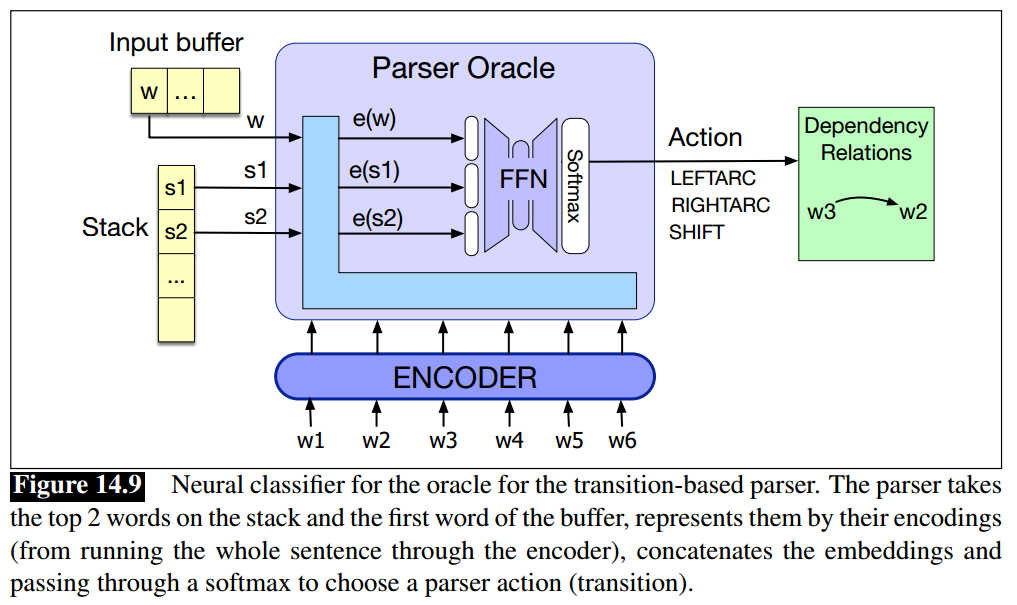
\includegraphics[scale = 0.4]{neural_transit_dep_parse.png}}
\end{minipage}
\caption{\footnotesize{\textbf{The neural network as oracle in transit-based dependency parsing}.}}
\label{fig: neural_transit_dep_parse}
\end{figure}

\subsection{Advanced Methods in Transition-Based Parsing}
\begin{itemize}
\item The arc-standard transition system described above is only one of many possible systems. A frequently used alternative is the \textbf{arc eager transition system}. The arc eager approach gets its name from its ability to \emph{assert rightward relations much sooner} than in the arc standard approach.

\item The computational efficiency of the transition-based approach discussed earlier derives from the fact that it makes a single pass through the sentence, greedily making
decisions without considering alternatives. Of course, this is also a weakness – \emph{once a decision has been made it can not be undone}, even in the face of overwhelming
evidence arriving later in a sentence. We can use \textbf{beam search} to explore alternative decision sequences.

Beam search uses a \textbf{breadth-first search strategy} with a \emph{\textbf{heuristic filter}} that prunes the \emph{search frontier} to stay within a fixed-size \textbf{beam width}. 
\begin{itemize}
\item Instead of choosing the single best transition operator at each iteration, we’ll apply \textbf{all applicable operators} to each state on an agenda and then \textbf{score} the resulting configurations. 

\item We then \textbf{add each} of these new configurations to the frontier, subject to the constraint that there has to be room within the beam. As long as the size of the agenda is within the specified beam width, we can add new configurations to the agenda. 

\item Once the agenda reaches the limit, we only add new configurations that are \textbf{better} than \emph{the worst configuration} on the agenda (\textbf{removing} the worst element so that we stay within the limit). 

\item Finally, to insure that we retrieve the best possible state on the agenda, the while loop \textbf{continues} \emph{as long as there are non-final states} on the agenda
\end{itemize}

The beam search approach requires a more elaborate notion of scoring than we used with the greedy algorithm. The oracle's choice can be viewed as assigning a score to all the
possible transitions and picking the best one. Let $\text{Score}(t,c)$ is the score assigned by Oracle based on features from current configuration $c$ and operator $t$. In order to track the score for the entire history, we can define the score for a new configuration as the score of its predecessor plus the score of the operator used to produce it.
\begin{align*}
\text{ConfigScore}(c_0) &= 0.0\\
\text{ConfigScore}(c_i) &= \text{ConfigScore}(c_{i-1})+ \text{Score}(t_i, c_{i-1})
\end{align*} Figure \ref{fig: beam_search_dep_parse} describes the algorithm for beam search on dependency parsing.
\end{itemize}

\begin{figure}
\begin{minipage}[t]{1\linewidth}
  \centering
  \centerline{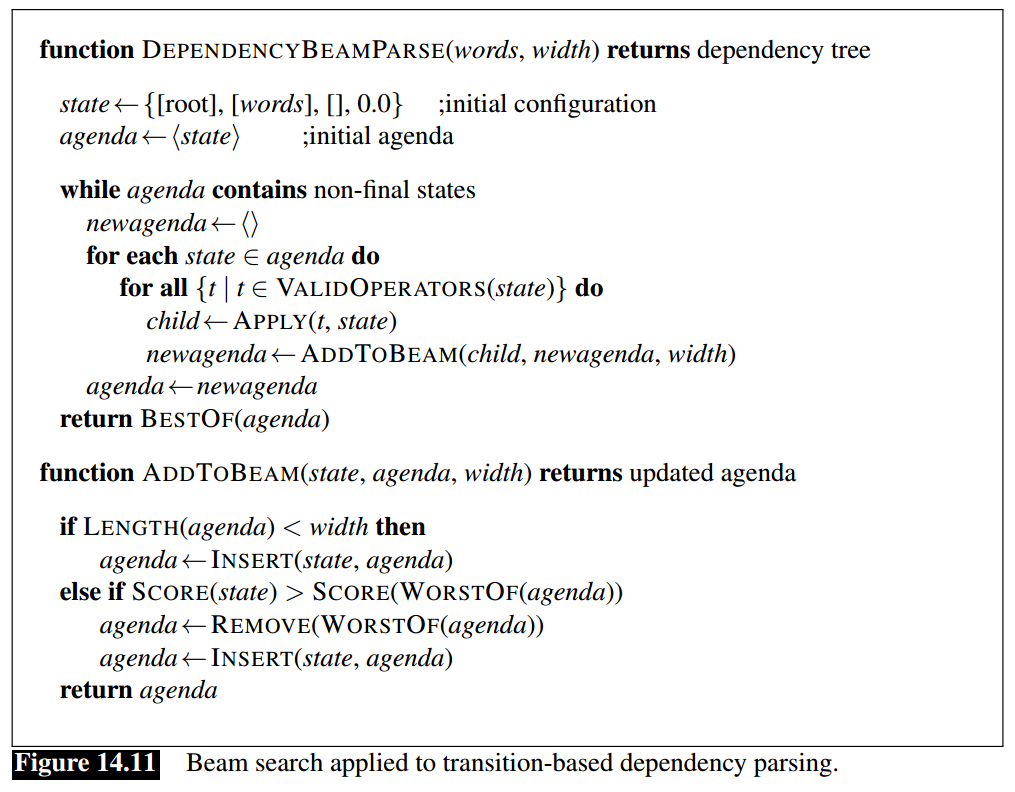
\includegraphics[scale = 0.4]{beam_search_dep_parse.png}}
\end{minipage}
\caption{\footnotesize{\textbf{The algorithm for beam search on dependency parsing}.}}
\label{fig: beam_search_dep_parse}
\end{figure}

\section{Graph-Based Dependency Parsing}
\begin{itemize}
\item \textbf{Graph-based parsers} are \emph{more \textbf{accurate}} than transition-based parsers, especially on long sentences;
\item Transition-based methods have trouble when the heads are \textbf{very far from the dependents}. Graph-based methods \textbf{avoid this difficulty by scoring entire trees}, rather than relying on greedy local decisions.

\item Furthermore, unlike transition-based approaches, graph-based parsers can produce \textbf{non-projective trees}. Although projectivity is not a significant issue for English, it is definitely a problem for many of the world’s languages.
\end{itemize}
  

Graph-based dependency parsers search through the space of possible trees for a given sentence for a tree (or trees) that \textbf{maximize some score}. These methods encode the search space as directed graphs and employ methods drawn from \emph{graph theory} to \emph{search} the space for optimal solutions. 

More formally, given a sentence $S$ we’re looking for the best dependency tree in $\cG(S)$, the space of all possible trees for that sentence, that maximizes some score:
\begin{align*}
\hat{T}(S) &= \argmax_{t \in \cG(S)}\text{Score}(t, S).
\end{align*} This score function is \textbf{edge-factored}, i.e. it can be decomposed into sum of scores on edges. 
\begin{align*}
\text{Score}(t, S) &= \sum_{e \in t}\text{Score}(e, S)
\end{align*}

Graph-based algorithms have to solve two problems:
\begin{enumerate}
\item assigning a score to each edge, 
\item finding the best parse tree given the scores of all potential edges.
\end{enumerate}

\subsection{Parsing via finding the maximum spanning tree}
We \textbf{initialize} the graph $G$ as a fully connected, directed, weighted graph where the vertices are the input words and the directed edges represent \emph{all possible head-dependent assignments}. We also add a node \emph{ROOT} with outgoing edges directed at all of the other vertices. The edge weight reflects the score for each possible head-dependent relation assigned by some algorithm.

The optimal dependent tree can be found via \textbf{maximum spanning tree} over $G$. A spanning tree over a graph G is a subset of $G$ that is a tree and covers all the vertices in $G$; a spanning tree over $G$ that \emph{starts} from the ROOT is a \emph{valid parse} of $S$. A maximum spanning tree is the spanning tree with the \textbf{highest score}. Thus a maximum spanning tree of G emanating from the ROOT is the optimal dependency parse for the sentence.

Some intuitions on the spanning tree and directed graph:
\begin{itemize}
\item Every vertex in the spanning tree has \textbf{exactly one} incoming edge. This is because every connected components of a spanning tree will only have one incoming edge. 
\item The absolute values of the edge scores are not critical in determining the maximum spanning tree. It is the relative weights of the edges entering each vertex matters. Therefore, the tree structure will be maintained if all edges entering a vertex have subtracted a constant.    
\end{itemize}

\begin{figure}
\begin{minipage}[t]{1\linewidth}
  \centering
  \centerline{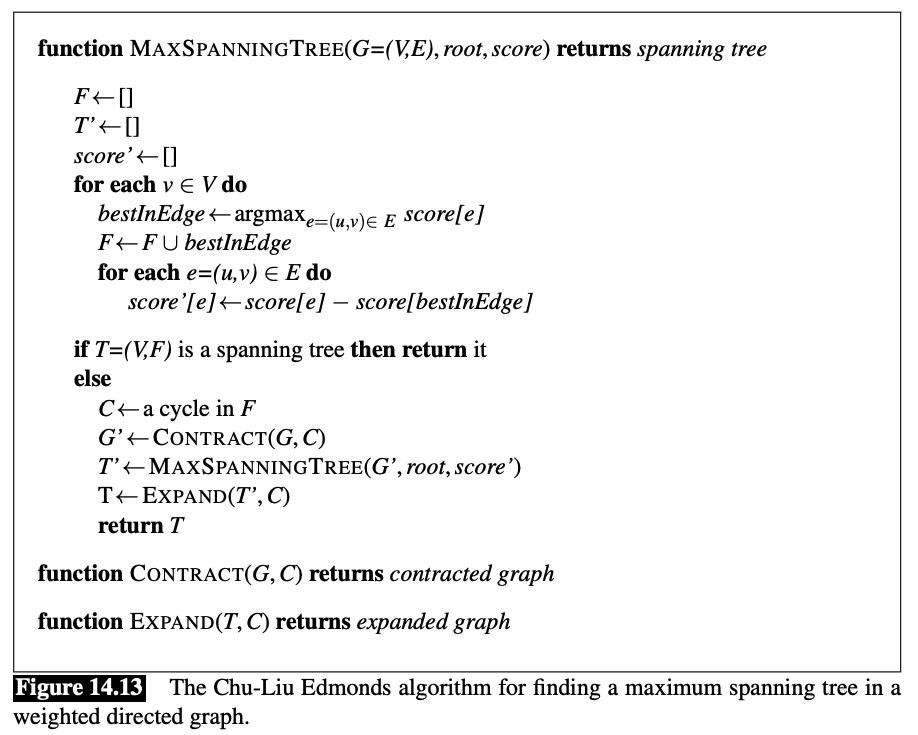
\includegraphics[scale = 0.4]{max_spanning_tree_depend_parse.png}}
\end{minipage}
\caption{\footnotesize{\textbf{The algorithm for finding the maximum spanning tree on dependency parsing}.}}
\label{fig: max_spanning_tree_depend_parse}
\end{figure}

The algorithm for searching the maximum spanning tree is described in Figure \ref{fig: max_spanning_tree_depend_parse} \citep{chu1965shortest} and \citep{edmonds1968optimum}. 
\begin{enumerate}
\item \textbf{The greedy edge selection phase}: The first step is to choose the incoming edge with the highest score. (i.e. greedy search finding the best head assignment for given dependent.) If the resulting set of edges are spanning tree, then we have obtained the maximum spanning tree. 

\item \textbf{The weight adjustment/re-scoring phase}: If the resulting edges contain circles, we need to eliminate some of these edges to break the circle. The cleanup phase begins by adjusting all the weights in the graph by \textbf{subtracting the score of the maximum edge entering each vertex} from the \emph{score of all the edges entering that vertex}. For the weight of edges in the circle, they have no bearing on the weight of \emph{any of the possible spanning trees}, since it will result in a weight of zero for all edges selected during the greedy selection phase, including all edges in the circle.

\item \textbf{The node collapsing phase}: Having adjusted the weights, the algorithm creates a new graph by selecting a
cycle and \textbf{collapsing} it into a single new node. Edges within the circle will be dropped and only edges connect to the circle remains. The other edges also are unchanged. This results in a new graph.

\item \textbf{The recursive cleanup phase}: Now we recursively find the maximum spanning tree on the new graph. The edge of the maximum spanning tree directed towards the vertex representing the collapsed cycle tells us which edge to delete to eliminate the cycle. When each recursion completes we \textbf{expand the collapsed vertex}, restoring all the vertices and edges from the cycle with the exception of the single edge to be deleted.
\end{enumerate}
We can see the example running this algorithm in Figure \ref{fig: max_spanning_tree_example}. The \textbf{time complexity} of the \textbf{Chu-Liu Edmonds (CLE) algorithm} (\citep{chu1965shortest} and \citep{edmonds1968optimum}) is $\cO(mn)$ where $m$ is number of edges and $n$ is the number of nodes. Since we begins with fully connected graph $m=n^2$, the total time complexity is $\cO(n^3)$. A more efficient algorithm from \citep{gabow1986efficient} could reach to $\cO(m + n\log n)$.

\begin{figure}
\begin{minipage}[t]{1\linewidth}
  \centering
  \centerline{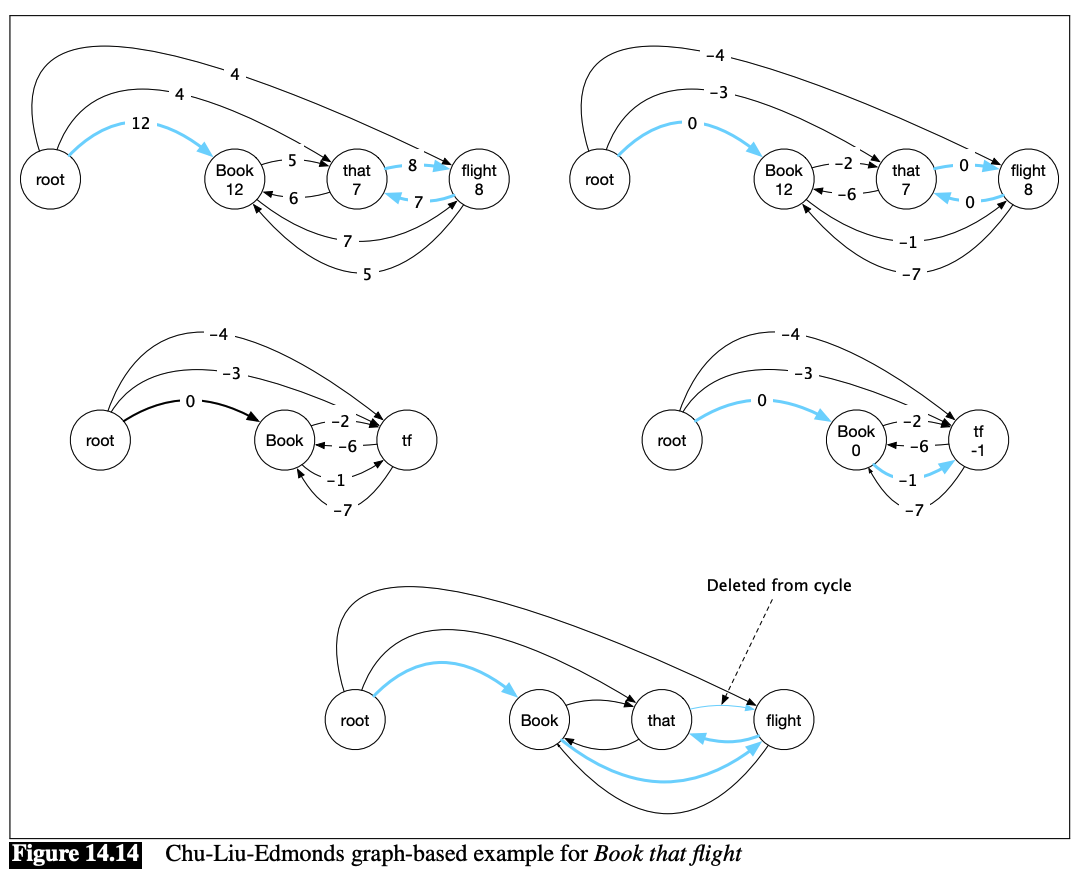
\includegraphics[scale = 0.4]{max_spanning_tree_example.png}}
\end{minipage}
\caption{\footnotesize{\textbf{The example for maximum spanning tree search. The blue edges are selected using greedy search for each vertex and the score are re-normalized based on the selected edge score}.}}
\label{fig: max_spanning_tree_example}
\end{figure}

\subsection{A feature-based algorithm for assigning scores}
Note that the score for the tree is the sum of scores of the edges within the tree. 
\begin{align*}
\text{Score}(t, S) &= \sum_{e \in t}\text{Score}(e, S)
\end{align*}

In a feature-based algorithm we compute the edge score as a weighted sum of features extracted from it:
\begin{align*}
\text{Score}(e, S) &= \sum_{j=1}^{N}w_{j}f_{j}(e, S)
\end{align*} where $[f_{j}]_{1,\ldots,N}$ are a set of features based on 
\begin{itemize}
\item \emph{Word forms}, \emph{lemmas},  \emph{parts of speech} of head, its dependent,
\item \emph{Word embeddings}.
\item the Corresponding features from the \emph{contexts} before, after and between the words., 
\item the \emph{dependency relation to the head}.
\item The \emph{direction of the relation} (to the right or left)
\item The \emph{distance} from the head to the dependent
\end{itemize}
 They are the same features used to define the training data for transit-based parser in Section \ref{sec: feature_classifier}. These features can be pre-selected or generated using feature templates. 

To learn a set of weights for these features, we train a model that assigns higher scores to correct trees than to incorrect ones. (unlike in Section \ref{sec: train_model} where we need the class labels as well as parse actions in training set.) An effective framework for problems like this is to use \textbf{inference-based learning} combined with the perceptron learning rule. In this setting, we initialize the weight randomly and use it to parse the training sentences. If the resulting parse matches the corresponding tree in the training data, we do nothing to the weights. Otherwise, we find those features in the \textbf{incorrect parse} that are \emph{not present in the reference parse} and we \textbf{lower their weights} by a small amount based on the learning rate. (\textbf{online learning})  We do this incrementally for each sentence in our training data until the weights converge.

\subsection{Using neural network for assigning scores}
The state-of-the-art algorithm uses the neural network to assign scores. Instead of extracting hand-designed features to represent each edge between words $w_i$ and $w_j$, these parsers run the sentence through an \emph{encoder}, and then pass the encoded representation of the two words $w_i$ and $w_j$ through a network that estimates a score for the edge $i \rightarrow j$. Figure \ref{fig: nn_score_asigning_dep_parse} shows one type of architectures. 

\begin{figure}
\begin{minipage}[t]{1\linewidth}
  \centering
  \centerline{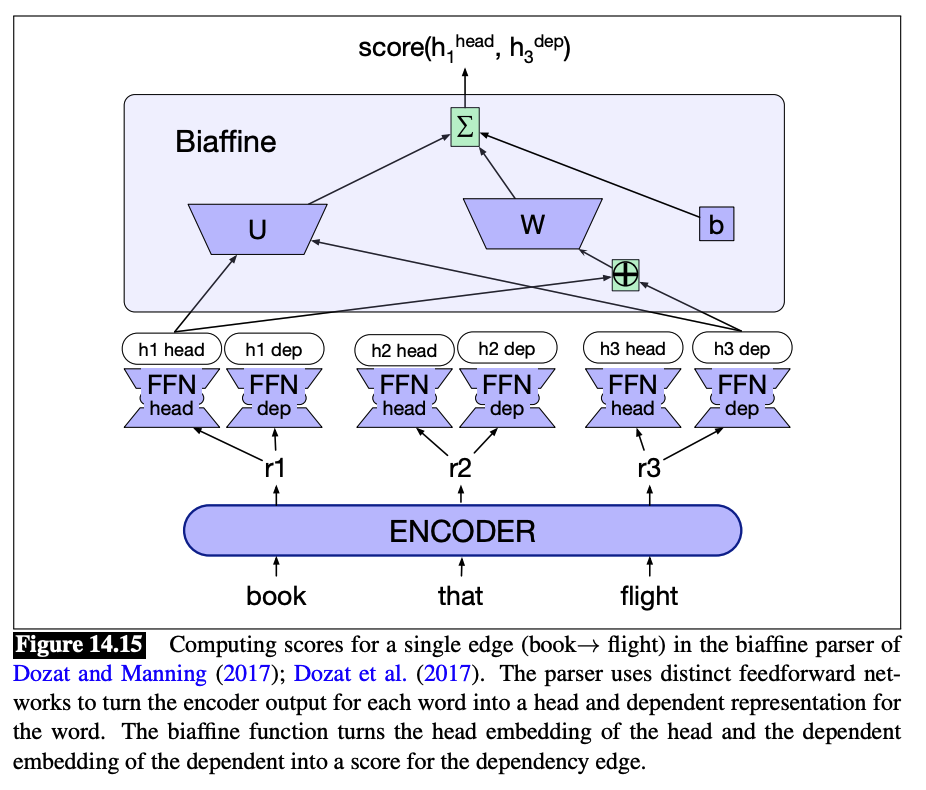
\includegraphics[scale = 0.4]{nn_score_asigning_dep_parse.png}}
\end{minipage}
\caption{\footnotesize{\textbf{The neural network based score assignment. The neural network uses encoder to learn weight between words based on the the word embedding of two vertices}.}}
\label{fig: nn_score_asigning_dep_parse}
\end{figure}

In the network, there are two feed-forward networks for each word: one to produce representation as a head, the other one to produce representation as a dependent. When we assign score from $i\rightarrow j$, we use the head representation for $w_i$ and the dependent representation for $w_{j}$ and passing them through an \emph{biaffine function} $\text{Biaff}(\mb{x}, \mb{y}):= \mb{x}^{T}\mb{U}\mb{y} + \mb{W}(\mb{x}\oplus \mb{y}) + b$. The idea of using a \textbf{biaffine scoring function} is allow the system to learn multiplicative interactions between the vectors $\mb{x}$ and $\mb{y}$. Finally we can pass the score function to a softmax to obtain probabilities. $p(i\rightarrow j) = \text{softmax}([\text{Score}(k\rightarrow j);, \forall k\neq j])$ . This probability can then be passed to the maximum spanning tree algorithm.

Note that the algorithm as we’ve described it is \emph{unlabeled}. To make this into a \emph{labeled} algorithm, \citep{dozat2016deep} proposes algorithm actually trains two classifiers. The first classifier, \textbf{the edge-scorer}, the one we described above, assigns a probability $p(i\rightarrow j)$  to each word $w_i$ and $w_j$. Then the Maximum Spanning Tree algorithm is run to get a single best dependency parse tree for the second. We then apply a second classifier, the \textbf{label-scorer}, whose job is to find the maximum probability label for each edge in this parse. This second classifier has the same form as (Figure \ref{fig: nn_score_asigning_dep_parse}), but instead of being trained to predict with binary softmax the probability of an edge \emph{existing} between two words, it is trained with a softmax over
dependency labels to \textbf{predict the dependency label} between the words.



\newpage
\bibliographystyle{plainnat}
\bibliography{book_reference.bib}
\end{document}